%%% template.tex
%%%
%%% This LaTeX source document can be used as the basis for your technical
%%% paper or abstract.

%%% The parameter to the ``documentclass'' command is very important.
%%% - use ``review'' for content submitted for review.
%%% - use ``preprint'' for accepted content you are making available.
%%% - use ``tog'' for technical papers accepted to the TOG journal and
%%%   for presentation at the SIGGRAPH or SIGGRAPH Asia conference.
%%% - use ``conference'' for final content accepted to a sponsored event
%%%   (hint: If you don't know, you should use ``conference.'')

%\documentclass[review]{acmsiggraph}
%
%
%%import important libraries
%% Arabic page numbers for submission. 
%% Remove this line to eliminate page numbers for the camera ready copy
%\pagenumbering{arabic}
%
%
%% Load basic packages
%\usepackage{balance}  % to better equalize the last page
%\usepackage{graphics} % for EPS, load graphicx instead
%\usepackage{times}    % comment if you want LaTeX's default font
%\usepackage{url}      % llt: nicely formatted URLs
%%\usepackage{lineno}
%%\linenumbers
%
%%\usepackage{cite}
%\graphicspath{ {./images/} }
%\usepackage{array}
%
%
%%for underline
%\usepackage[normalem]{ulem}
%
%%colours
%\usepackage[usenames]{xcolor}
%\usepackage{colortbl}
%\definecolor{tableheadercolor}{gray}{0.95}
%
%% create a shortcut to typeset table headings
%\newcommand\tabhead[1]{\small\textbf{#1}}
%
%
%%used to label TODOs
%\newcommand\todo[1]{\textbf{\textcolor{red}{TODO:} \textit{#1}}}
%
%% KM - for comments
%\newcommand{\inlinecomment}[3][]{$\lceil$\textbf{#1}~\textit{\textcolor{#2}{#3}}$\rfloor$}
%\definecolor{DarkGreen}{rgb}{0.0, 0.5, 0.0}
%\definecolor{DarkRed}{rgb}{0.7, 0.2, 0.2}
%\definecolor{DarkOrange}{rgb}{1, 0.5, 0}
%\definecolor{Orange}{rgb}{1, 0.75, 0}
%
%
%\newcommand{\kmC}[1]{\noindent \inlinecomment[KM]{DarkGreen}{#1}}
%\newcommand{\kmE}[1]{\textcolor{DarkRed}{#1}}
%
%\newcommand{\osC}[1]{\noindent \inlinecomment[OS]{Orange}{#1}}
%%\newcommand{\osC}[1]{}
%\newcommand{\osE}[1]{\textcolor{DarkOrange}{#1}}


\newcommand{\qq}[2]{\emph{``#1"} (#2)}
\newcommand{\HAtheme}[2]{\textbf{Theme #1:} \uline{#2}\\}




%%% Make the ``BibTeX'' word pretty...

%\def\BibTeX{{\rm B\kern-.05em{\sc i\kern-.025em b}\kern-.08em
%    T\kern-.1667em\lower.7ex\hbox{E}\kern-.125emX}}
%
%%%% Used by the ``review'' variation; the online ID will be printed on 
%%%% every page of the content.
%
%\TOGonlineid{0560}
%
%%%% Used by the ``preprint'' variation.
%
%\TOGvolume{0}
%\TOGnumber{0}
%
%\title{Design of a Haptic Animation Tool for Grid Displays}
%
%\author{Oliver Schneider\thanks{e-mail:spencer@cs.washington.edu}\\University of British Columbia
%\and Ali Israr\thanks{e-mail:israr@disneyresearch.com}\\Disney Research
%\and Karon Maclean\thanks{e-mail:spencer@cs.washington.edu}\\University of British Columbia
%}
%\pdfauthor{Oliver Schneider}
%
%\keywords{Haptic media; vibrotactile arrays; authoring tools.}
%
%\begin{document}
%
%%% This is the ``teaser'' command, which puts an figure, centered, below 
%%% the title and author information, and above the body of the content.


%\maketitle

\chapter{Manipulate: Tactile Animation}
\label{ch:hapticanimation}

  % \teaser{
\begin{figure}[h]
   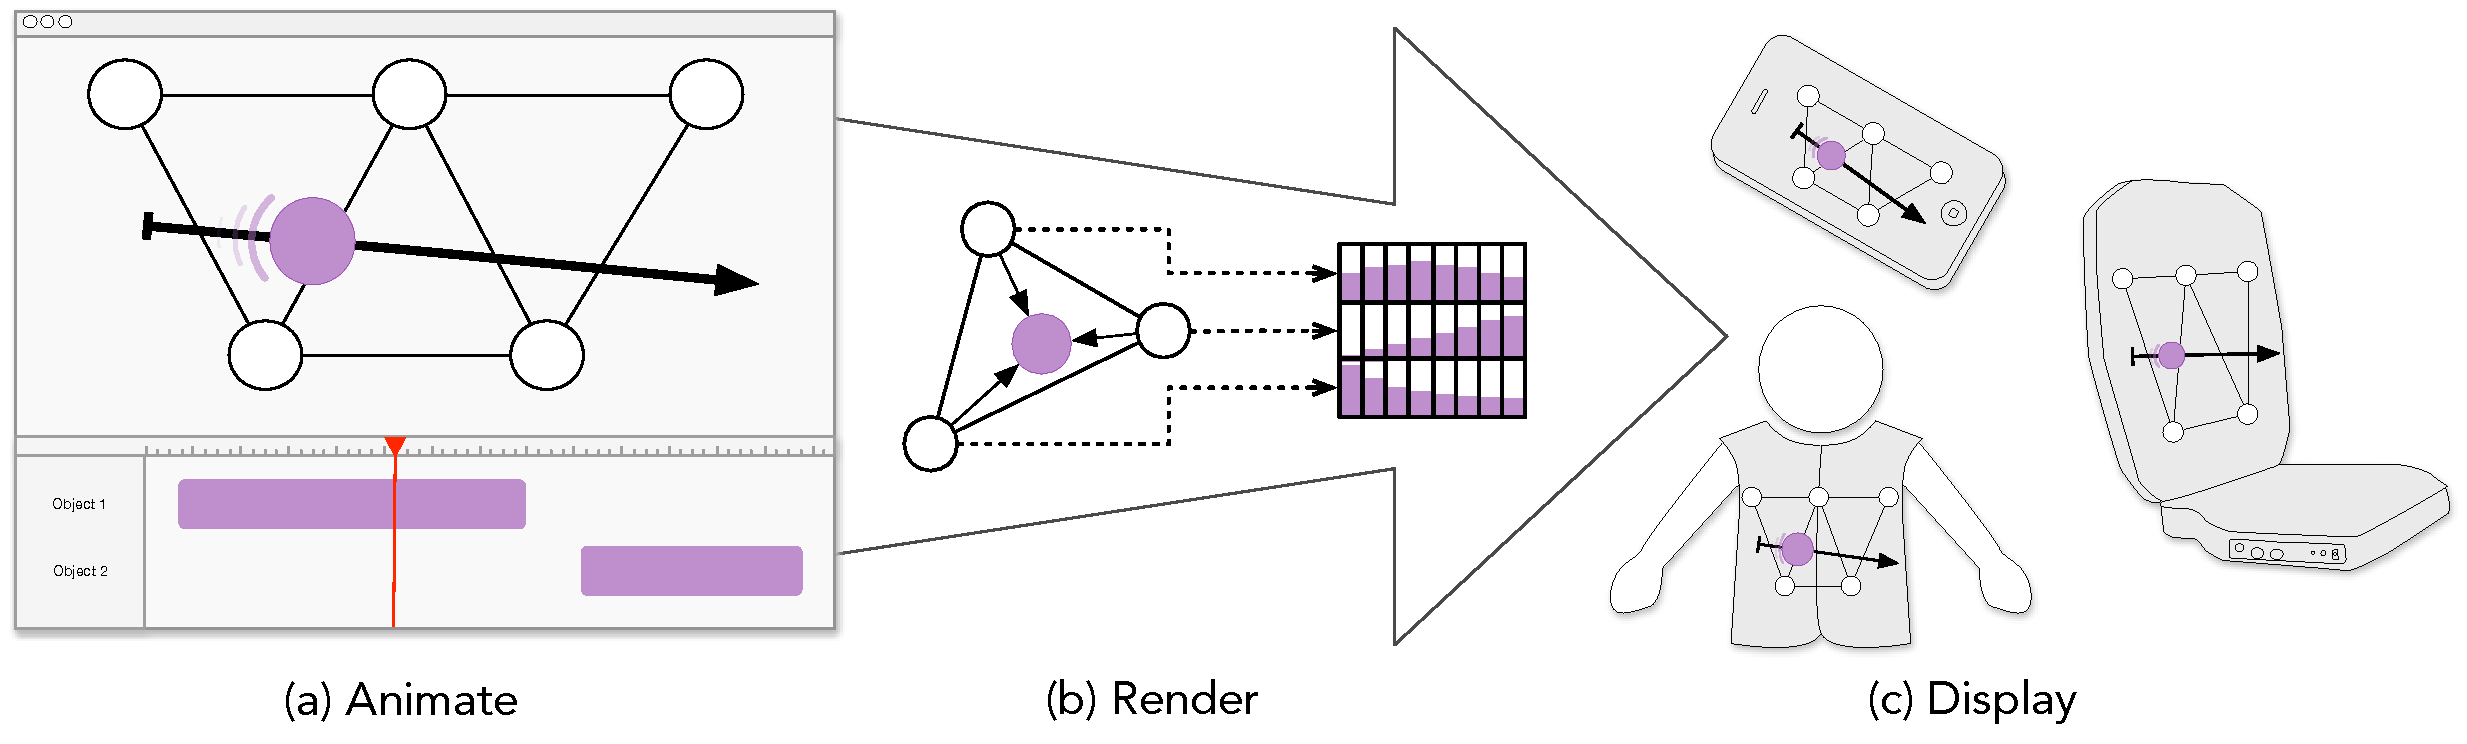
\includegraphics[width=0.98\textwidth]{images/HA14-Concept-Sketch-2015-01-17-1127}
   \caption{Concept sketch for tactile animation. 
An artist draws an animated sequence in the user interface and the user experiences phantom 2D sensations in-between discrete actuator grids. 
%The animator controls phantom sensations directly, without needing to think in device terms, and designs expressive sensations for arbitrary vibrotactile arrays.
}
   \label{fig:concept:sketch}
\end{figure}
% }

  

%Chairs, wearables, and handhelds have become popular sites for spatial tactile display.
%Visual animators, 
%already expert in using time and space to portray motion, could readily transfer their skills to production of rich haptic sensations if given the right tools.
In this second case study, we iterate on some of our findings from the haptic instrument to design a full authoring tool, using real-time feedback but supporting refinement with time-based editing.
This work\footnote{In peer review at the time of this writing.} targeted professional media designers (especially animators) creating spatial vibrotactile sensations.
To afford real-time manipulation, we developed the \emph{tactile animation object}, a persistent, manipulable primitive rendered through phantom vibrotactile sensations, and implement Mango, an editing tool built for animators.
%We describe Mango's interface, rendering pipeline, and perceptually-optimized interpolation algorithm.
In our evaluation,
professional animators found it easy to create a variety of
vibrotactile patterns, with both experts and novices preferring the tactile animation object over
controlling actuators individually.
Furthermore, the tactile animation metaphor is a generalizable concept that can extend to several devices.
%, which we explore before concluding.
%in authoring real-time feedback on a variety of grid displays.

  

  
%%%%%%%%%%%%%%
%
% Section - Intro
%
%%%%%%%%%%%%%%
%\section{Introduction}

%Haptic feedback is % increasingly 
%viewed in today's entertainment and media industry as a key ingredient of immersive experience.
%%%whose potential has not been unlocked.
%Motion platforms and large shakers appear in theater seats, ride vehicles, and gaming platforms to tilt, rotate, translate and shake the user's body to build engagement and fun.
%A new genre of haptic technologies aim to supplement movies, games, and even users' social activities with expressive and synchronized cues at multiple locations on the skin
%\cite{Israr2011,Danieau2012a,Sodhi2013,Kim2009}. 
%Similar opportunities await well-designed wearable and handheld displays.
%Unfortunately, adoption has been limited by the dearth of authoring tools for generating rich sensory content.
%
%
%%Critically, this haptic content is crafted, tested, synchronized and stored during media production using custom software plugins made for tools familiar to  media designers and artists,
%%requiring little modification to existing production pipelines. 
%%In this paper we present, implement, and evaluate key elements of a haptic authoring system that allows artists and designers to quickly generate spatio-temporal haptic media on multi-actuator haptic technologies. 
%
%Multi-actuator vibrotactile (VT) arrays,
%which stimulate the skin through vibration, appear in diverse applications and form factors, from chair-based immersive gaming  \cite{Israr2011} to wearable vests for mobile awareness \cite{Jones2004}.
%%To create expressive sensations, however, designers typically must be programmers and haptic experts.
%%Several device-specific tools for prototyping or final authoring of haptic sensations have introduced user-friendly and user-familiar interfaces. 
%Most VT authoring tools only support a single actuator \cite{Enriquez2003}; those that accommodate multiple actuators % deleted Lee2009
%control each separately \cite{Kim2009,Paneels2013,Swindells2014}.
%These multitrack authoring tools %allow designers to edit, test, and save time-series data for individual actuators, but
%are cumbersome and complicated for systems having as many as % greater than 
%%10 or 20 vibrating actuators (e.g., one haptic jacket for movie goers is equipped with 
%64 vibrators \cite{Jones2009}.
%%). %(Tactile 
%
%{\it Direct manipulation} of a spatial animation object provides
%%rather than by coordinating multiple tracks. 
%a simpler mental model that eases the transition of visual animators into haptic design.
%We build on the notion of a phantom vibration perceived in-between physical actuators \cite{Alles1970,Israr2011a} to support real-time spatiotemporal tactile feedback in sparse actuator arrays, enabling direct manipulation.
%Specifically, we present the %concept of a 
%\textbf{tactile animation object}, a visualized abstract phantom sensation, and implement it in \emph{Mango}, a tactile animation tool and rendering pipeline (\autoref{fig:concept:sketch}).
%
%
%Our contributions are: 
%%We have three contributions.
%1)  A tactile animation interface grounded in user interviews and prior literature.
%% The design is derived from interviews and prior literature, ..  includes tools 
%%Derived from interviews and prior literature, its design integrates techniques familiar to a mainstream animator workforce. 
%2) A rendering pipeline translating tactile animation objects %designed % animated 
%%haptic patterns to sparse VT arrays, and optimize its rendering algorithm with a user study.
%to phantom sensations on sparse, generalized VT arrays, optimized with a perceptual study.
%% We conduct a study to determine an optimal rendering algorithm for sparse VT arrays. 
%3) An evaluation with professional animators showing accessibility and expressivity.
%4) An exploration of the potential applications supported by tactile animation.
%% with \kmC{SLC} % in  ??? 
%%natural user gestures.
%% KM 04.12: at this point, 'animation metaphor' as connected to 'natural user gestures' is unclear - you haven't mentioned gestures yet so this comes out of nowhere. Can you restate this contribution more plainly?
%

\newcommand\prevWorkWidth{1in}
\newcommand\prevWorkImageWidth{0.65in}


%\begin{figure}[b]
% \centering
%   \begin{subfigure}[t]{\prevWorkWidth}
%	  \centering
%	   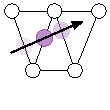
\includegraphics[width=\prevWorkImageWidth]{HA14-PreviousWork-TactileBrush-2015-04-12-1100} 
%	   \caption{Tactile Brush \cite{Israr2011a}: precomputed curves}
%	   \label{fig:prevwork:tactilebrush}
%    \end{subfigure}
%    ~
%  \begin{subfigure}[t]{\prevWorkWidth}
%  	\centering
%	   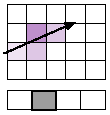
\includegraphics[width=\prevWorkImageWidth]{HA14-PreviousWork-TactileMovies-2015-04-12-1100} 
%	   \caption{Tactile Video \cite{Kim2009}: frames of tactile pixels}
%	   \label{fig:prevwork:tactilemovies}
%    \end{subfigure}
%    ~
%      \begin{subfigure}[t]{\prevWorkWidth}
%	      \centering
%	   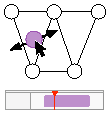
\includegraphics[width=\prevWorkImageWidth]{HA14-PreviousWork-HA-2015-04-12-1100} 
%	   \caption{Tactile Animation: direct manipulation}
%	   \label{fig:prevwork:ha}
%    \end{subfigure}
%    \caption{Comparison between related systems.}
%    \label{fig:prevwork}
%\end{figure}




%\begin{table*}
%	\begin{tabular}{|l|p{0.92\textwidth}|}
%	\hline
%	\rowcolor{tableheadercolor}
%
%	\textbf{LR}
%		%& \textbf{RW}
%		& \textbf{Description} \\
%	\hline
%		LR1 
%		 &
%		 \textbf{Real-Time Playback} \cite{Moussette2011,Schneider2014}
%		 Rapid prototyping is essential for working with VT sensations, especially in absence of objective metrics. % of success.
%		 Feeling a sensation at design time allows iteration to converge faster to better results. % and develop more engaging sensations.
%		 However, \textit{too} real-time can cause split attention.
%	\\
%	\hline
%		LR2 & 
%		 \textbf{Load, save, manipulate}
%		 \cite{Resnick2008,Johnson2002,Schneider2014}
%		 	A persistent object model is essential for sensation editing over % for being able to continue to work on sensations for 
%			longer projects and % for being able to share them 
%			sharing with other designers or across devices.
%			Well-defined actions upon a data structure also facilitates features like \textit{undo} that support experimentation.
%	\\
%	\hline
%		LR3 &
%		\textbf{Library of effects} \cite{Enriquez2003,Swindells2006,Herring2009,Paneels2013,Swindells2014}
%		% deleted Paneels2010
%			 A library of saved sensations is an important feature used in previous haptic authoring tools, providing inspiration and preventing designers from re-inventing the wheel.
%	\\
%	\hline
%		LR4 &
%		\textbf{Device configuration} \cite{Kim2009,Paneels2013,Lee2012,Lee2013}% deleted Lee2009
%			~Because of the many types of haptic devices, a general tool must be able to understand different devices.
%			Lightweight configuration files that describe each device are common in the literature.
%			The configuration file allows users to select specific hardware and specify location and type of actuators.
%			Animators can also select a rendering algorithm from a list of available ones.
%	\\
%	\hline
%		LR5 &
%		\textbf{Multiple channels \& combination of effects}
%		 \cite{Enriquez2003,Swindells2006,Ryu2008,Paneels2013,Swindells2014}	 
%		 Being able to display multiple effects simultaneously, or combine effects via superposition or concatenation, is essential for expanding the design space.
%		 This is typically represented in a timeline, which represents the temporal behaviour of any objects.
%	\\
%	\hline
%		LR6 &
%		\textbf{Visual/direct control metaphor}
%		\cite{Kim2009,Paneels2013,Cuartielles2012}
%		 Most previous tools consider each actuator separately.
%		 When thinking semantically about a spatial system, a direct view of the device and actuator layout is critical for direct manipulation.
%	\\
%	\hline
%		LR7 &
%		\textbf{Audio/visual context}
%		\cite{Kim2009,Swindells2014,Moussette2011}
%		 Haptic perception depends greatly on additional senses \cite{Hayward2008}. %cite hayward or pseudohaptics
%		By providing audio and visual feedback, these effects can be mitigated and the designer can experience haptic sensations in context.
%	\\
%	\hline
%		LR8 &
%		\textbf{User Feedback}
%		 \cite{Schneider2014,Swindells2014}
%		 Receiving feedback from users, either by demonstration or A/B testing, is extremely valuable.
%	\\
%	
%
%	\hline
%	\end{tabular}
%	\caption{{\bf Literature Requirements (LRs)} for a tactile animation authoring  tool.}
%	\label{tab:design:literature:requirements}
%\end{table*}



%%%%%%%%%%%%%%
%
% Section - Requirements Gathering
%
%%%%%%%%%%%%%%
\section{Mango, a Tactile Animation Authoring Tool}
% The objective of the haptic authoring tool 
To create a familiar and efficient % authoring
framework for  dynamic haptic content, we gathered two sets of requirements: Literature  (``LRs"), from prior research on haptic authoring tools, and Industry (``IRs") from interviews with five industry experts in haptic media creation and animation.
Our prototype, Mango, was built in  Python 2.7 and Tkinter (\autoref{fig:implementation:screenshot}),
communicating with a devices via USB.




%%%%%%%%%%%%%%
%
% Section - Framework
%
%%%%%%%%%%%%%%

%\subsection{Framework for Tactile Animation}
%%%%%%%%%%%%%%
%
% Framework for Haptic Animation


%In this section, we present an animation metaphor that allows users to generate tactile content in the same way as they would create visual animations and play them real-time on a VT array.
%\autoref{fig:feel:taxonomy} shows the workflow of this authoring mechanism.  
Designers create tactile animations on Mango as they would in a graphical animation tool. % as shown in \autoref{fig:feel:taxonomy}a.
The animation object is placed in space, and the designer adjusts % at a location and designers adjust 
its size on the visual outline of the VT array. %\kmC{SLC}. % KM 04.12: 'trace of a VT array" is unclear to me. 
% Once the object is created, they 
The designer then adds movements and special effects to the object using Mango's toolset,
% a set of tools provided in the Mango interface, 
and play it to observe timing. % of the animation. 

Mango's rendering engine translates visual animations to tactile animations on the VT array
%Knowing the location of vibrating points on the coarse array of VT actuators, the rendering engine resolves the animated sequence into individual actuators using the phenomena of phantom tactile sensations \cite{Alles1970,Israr2011a}. 
%The phantom sensation is a sensory illusion elicited by stimulating two or more vibratory elements on the skin.
%Instead of feeling the individual vibration points, the user feels a single sensation in between, whose perceived intensity is defined by the weighted sum of the intensities of the vibrating elements.
%Therefore, in each frame, the animated tactile object is resolved into intensity of actuators on the VT array (\autoref{fig:feel:taxonomy}b) .
%The rendering engine then calculates raw waveforms for each VT channel (\autoref{fig:feel:taxonomy}c) that can either be sent to the VT device to play the animated sequence or exported as a multichannel datafile for later use.
%Previous work has interpolated between only two actuators \cite{Seo2010,Lee2012a}; % KM 04.12 missing ref?
%however, a more generalized 3-actuator interpolation algorithm allows for arbitrary real-time manipulation of the tactile animation object on grid displays. 
%, but is less understood perceptually. As such, we guide our rendering algorithm with a perceptual study.
% presents additional challenges, including choosing a suitable rendering function
%OS: Should we explain that previous work has only interpolated between two actuators? Or would that invite questions about whether it feels right?
% KM: I think you risk this coming up if you don't.
%
% COMMENTED OUT JAN16 2:30PM PST
%
% all chan
%
%Several methods
%
%called \emph{vector sensations} (\autoref{fig:feel:taxonomy}(b)), 
%
%and each vector represents variation in intensity of the corresponding actuator of the VT array. From these vector sensations, the rendering engine calculates the raw waveform, called \emph{raster sensation}, at each sample instant for haptic rendering (\autoref{fig:feel:taxonomy}(c)). The sample rate for haptic rendering is usually faster than the frame rate and raster sensations are combination of intensity variations (vector sensations) and the stimulation frequency. These raster sensations are then sent to the haptic devices (\autoref{fig:feel:taxonomy}(d)) t
%To accommodate the animation framework, we define
using three {\bf datatype models}:
%for use in the current implementation and  future expansion of the Mango tool:
% if tight on space, following sentence is redundant with remainder of section since full refs are on same page.
\emph{Tactile animation objects}, high-level hardware-independent data types for tactile animation;
\emph{vector formats}, high-level hardware-specific control common in previous work; and
\emph{raster formats}, low-level hardware-specific formats for rendering and playback.
Data types are stored as JavaScript Object Notation (JSON) files.

%\textbf{Tactile animation objects} % KM: could save sig space by defining acronomym, given # of appearances.
%are high-level specifications of virtual sensations moving on a 2D VT array (\autoref{fig:feel:taxonomy}a).  
%High-level parameters, such as location, size, and other semantic qualities, can either be constant or variable. % interpolation methods. 
%Each tactile object has a start time and a duration.
%Object type is also defined for tactile animations that sets pre-defined parameters and features to animated objects. 
%For example, a moving virtual point can have a position, size, and frequency parameter; while a ``rain" effect has a position and more semantic parameters like raindrop frequency or size.
%
%%Similarly to visual effects present in animation tools like Adobe After Effects, each animation type is pre-programmed with various parameters and shown as tracks in timeline.
%%The detailed implementation of different animation object types is left for future expansion of Mango.
%
%Tactile animation objects are device-independent.
%Mango uses a device configuration file (LR4) and the rendering engine to create animated VT patterns on hardware.
%Animation objects can be combined in novel ways, organized in groups, or generate other tactile animations like a particle generator as in a graphical animation tool, and can have paths that constrain motion to a pre-determined trajectory.
%We prototyped an early version of the tactile animation object in Mango; however, the data type is extensible.% for future expansion. 
%

\begin{figure}[tbh] %  figure placement: here, top, bottom, or page
   \centering
   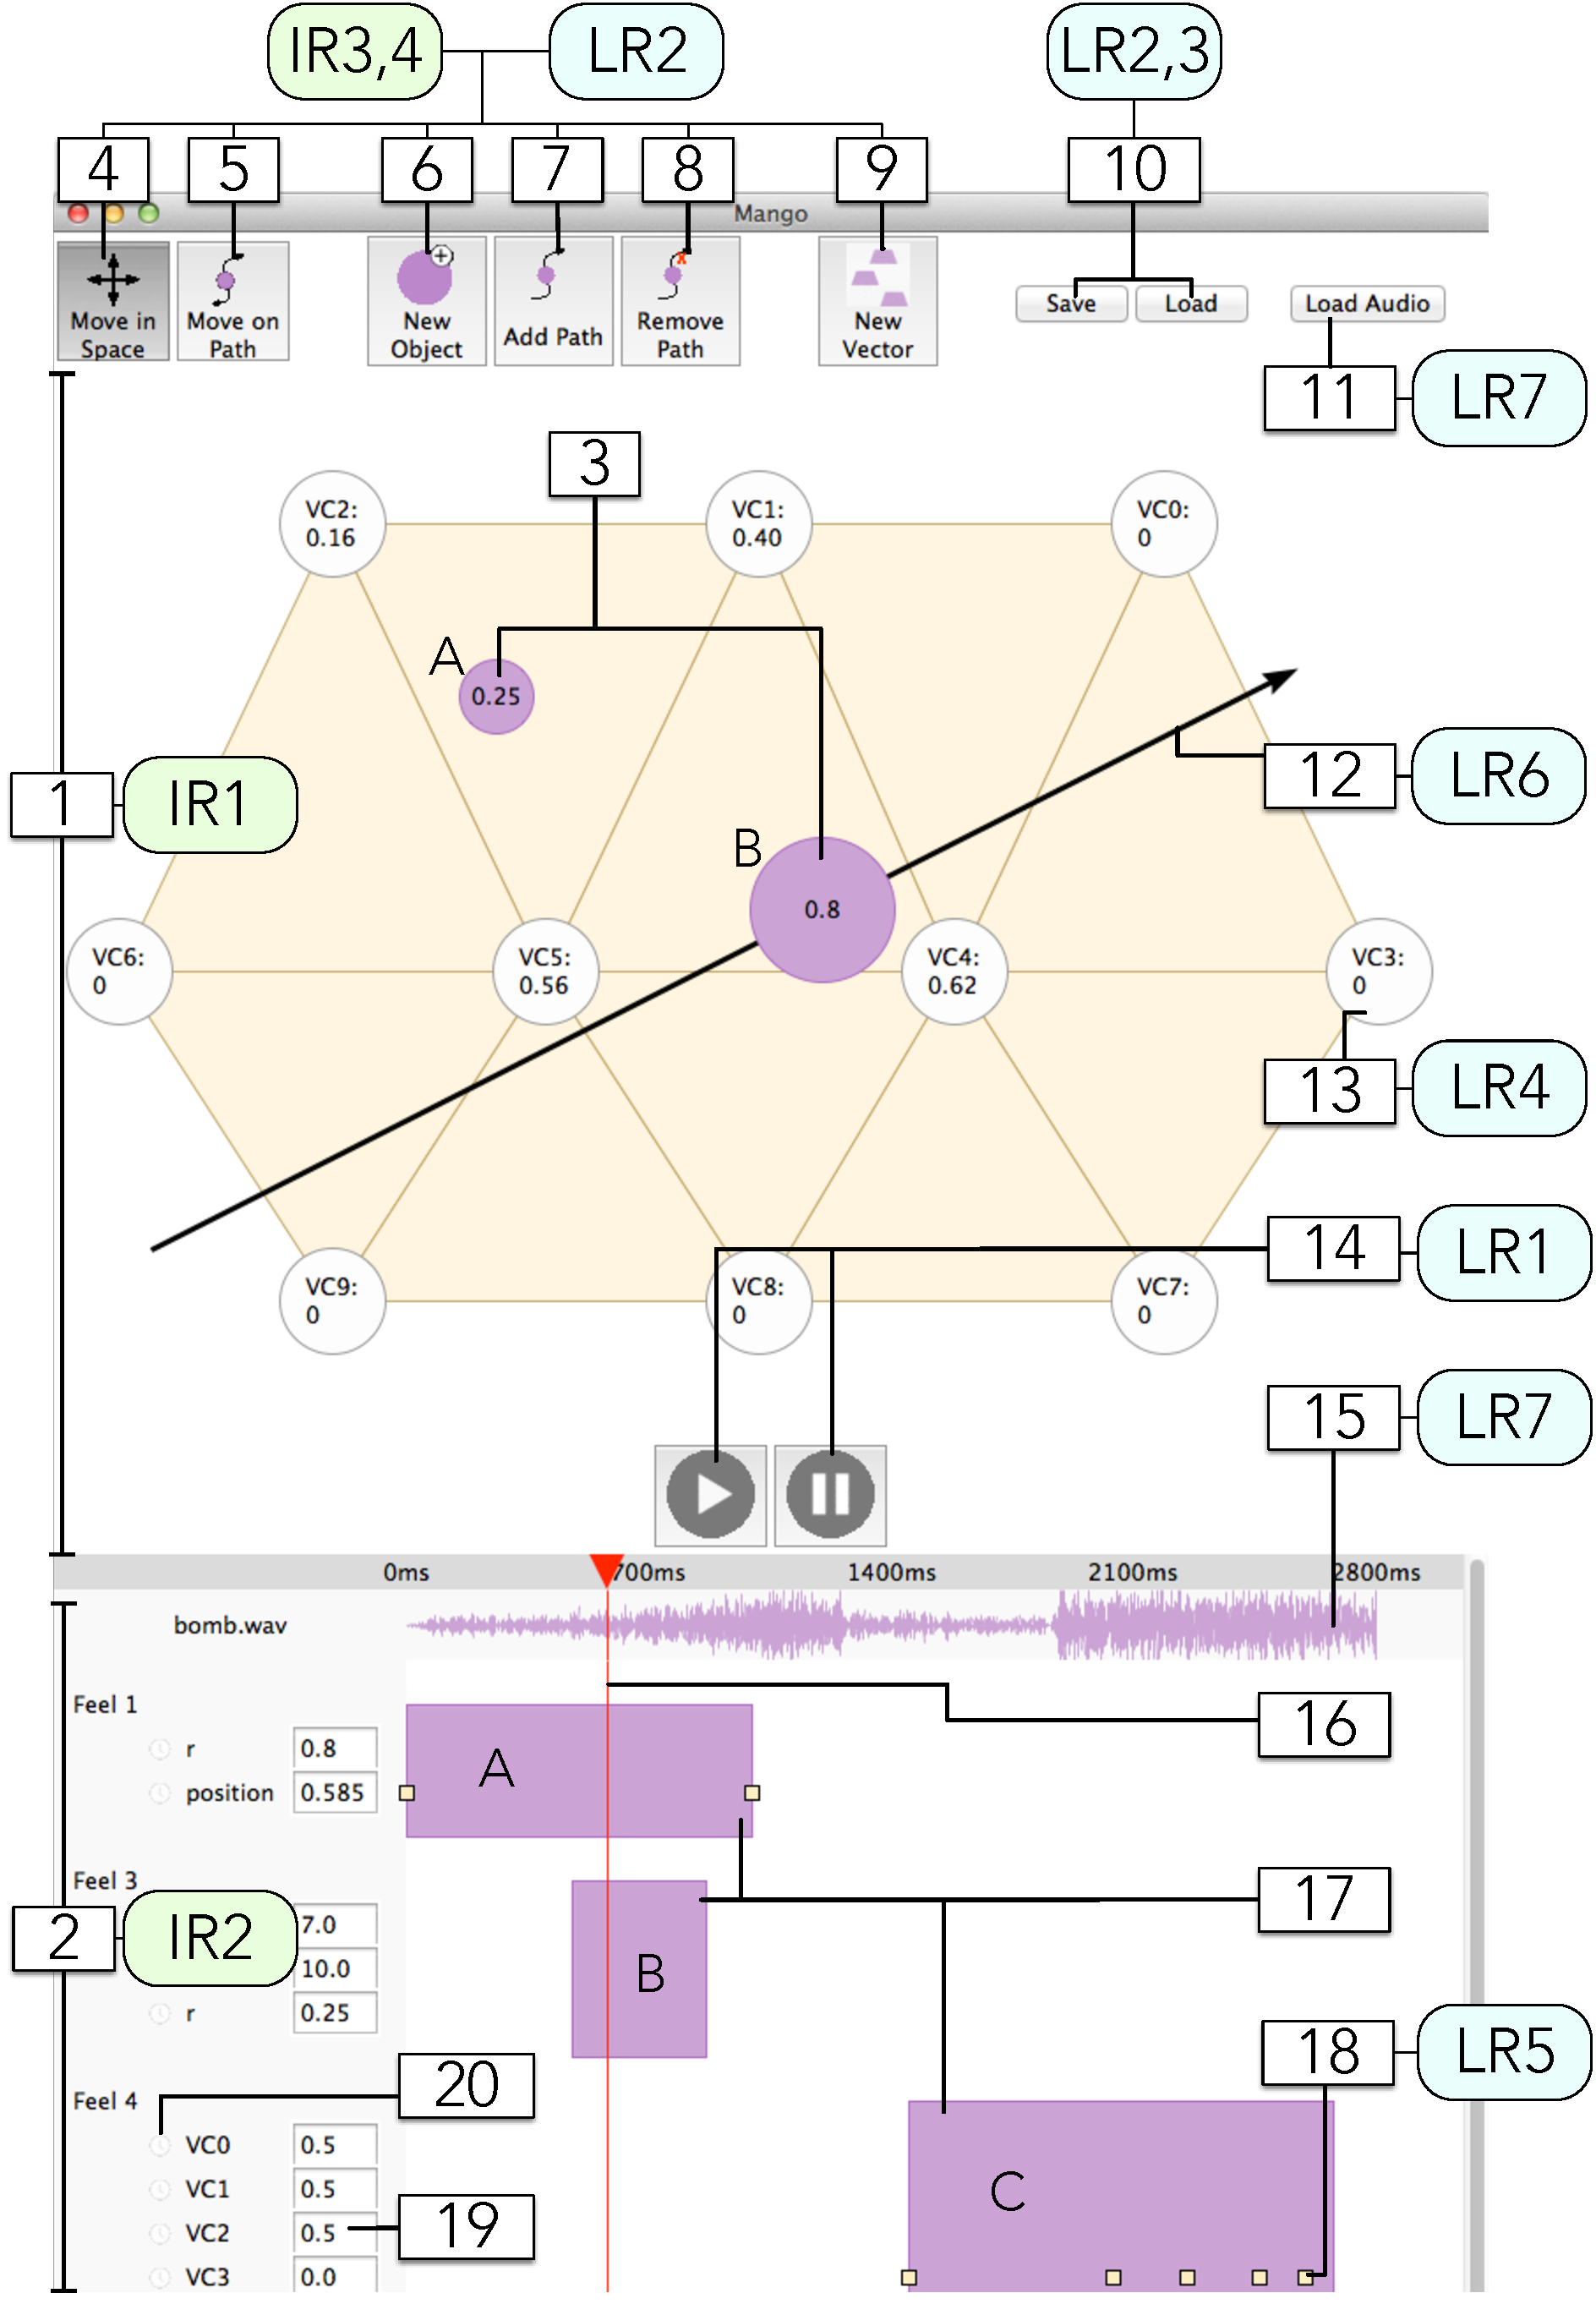
\includegraphics[width=0.47\textwidth]{Mango-Screenshot-Labeled-2015-04-12-1132} 
   \caption{Mango graphical user interface. Key components are labeled and linked to corresponding design requirements (LRs and IRs, not described in this proposal).}
   \label{fig:implementation:screenshot}
\end{figure}


%%%%%%%%%%%%%%%
%%
%% Section - Design
%%
%%%%%%%%%%%%%%%
%\subsection{Authoring Interface}
%%%\ALIc we need a good introductory sentense for this section.
%The authoring interface % is the key component in the Mango tool and % KM: so is the rendering pipeline isn't it?
%allows designers to efficiently create moving tactile content in a familiar environment.
%Here we describe user interactions to generate animated tactile content and associate them with our gathered design requirements. 
%% gathered in Section 3. 
%% In Mango's implementation, 
%Most Mango interactions are through the animation window (1) and  timeline (2) .
%%


%%%%%%%%%%%%%%
%
% Rendering Pipeline
%
%%%%%%%%%%%%%%
\section{Rendering Algorithm}
Mango's rendering algorithm translates animations in the animation window to animated VT patterns on the hardware.
%\autoref{fig:feel:taxonomy} shows the rendering pipeline that converts animation objects to vector sensations and a raster format, which outputs to the hardware.
The rendering algorithm
%is derived from %deep and extensive \kmC{SLC} % KM 04.12: are you sure about "deep/extensive"? sounds funny to me.
%psychophysical understanding of VT illusions on the skin and creates percepts of virtual actuators and their motion in between a set of real actuators.
%The precise perceptual model depends on several factors, such as type of VT actuators (DC vs. voice coil motors), stimulation site (forearm vs. back) and the spacing of actuators in the array (e.g., \cite{Israr2011a}).
%To allow for custom framerates and real-time feedback, we
generalizes from 1D phantom sensations (between two VT actuators along a line \cite{Seo2010,Alles1970,Israr2011a}) to 2D (between 3 or more actuators, \autoref{fig:rendering:algorithm:barycentric}).
%Thorough investigation of the psychophysical model is beyond our present scope; however, we empirically determine 
%the most effective model among those  % optimal model that is derived from various methods
% documented in the literature for the 1D case.
 %\kmC{2D vs 1D, slc} % KM: don't you need to go into more detail on 2D vs 1D? this seems like it's hinting at something without saying it.
%
%Here we describe the interpolation models for rendering algorithm used in the prior literature, and a pairwise comparison user study to determined the optimal interpolation model for the Mango's rendering algorithm.

%\subsection{Algorithm}
%The rendering algorithm translates virtual percepts to a physical actuator grid.
%We first construct a Delaunay triangulation for all actuators to automatically define a mesh on the hardware grid.
%At each instant of rendering, we use barycentric coordinates of the virtual animation objects relative to a triangle defined by three real actuators (\autoref{fig:rendering:algorithm:barycentric}).
%Barycentric coordinates are scaled by an interpolation method to determine real actuator intensity.
We had to choose between three interpolation models from prior psychophysical understanding of phantom tactile sensations \cite{Alles1970} and propose them as candidates for the Mango tool:
% They are: 
(i) {\it linear}, 
(ii) {\it logarithmic (``log")}, and 
(iii) {\it Pacinian power (``power")} interpolation. 
%
%%In the linear interpolation model, barycentric coordinates are linearly related to actuation amplitude. In the log model, these coordinates are scaled logarithmically, as perceived intensity is related to physical vibration amplitude 
%%\cite{verrillo1992perception}. In the power model,  coordinates are coupled to the power (square of the amplitude) of vibrating stimulations \cite{verrillo1992perception}. 
%%Linear and log interpolation models have been used in the past to express either location or intensity respectively (but not both) of virtual sensations between two vibrators \cite{Seo2010,Alles1970}. A Pacinian power model was used in \cite{Israr2011a} to account for both location and intensity of virtual sensation between two vibrators.
%

\begin{figure}[t] %  figure placement: here, top, bottom, or page
   \centering
  \begin{subfigure}[b]{0.4\textwidth}
  	\centering
	   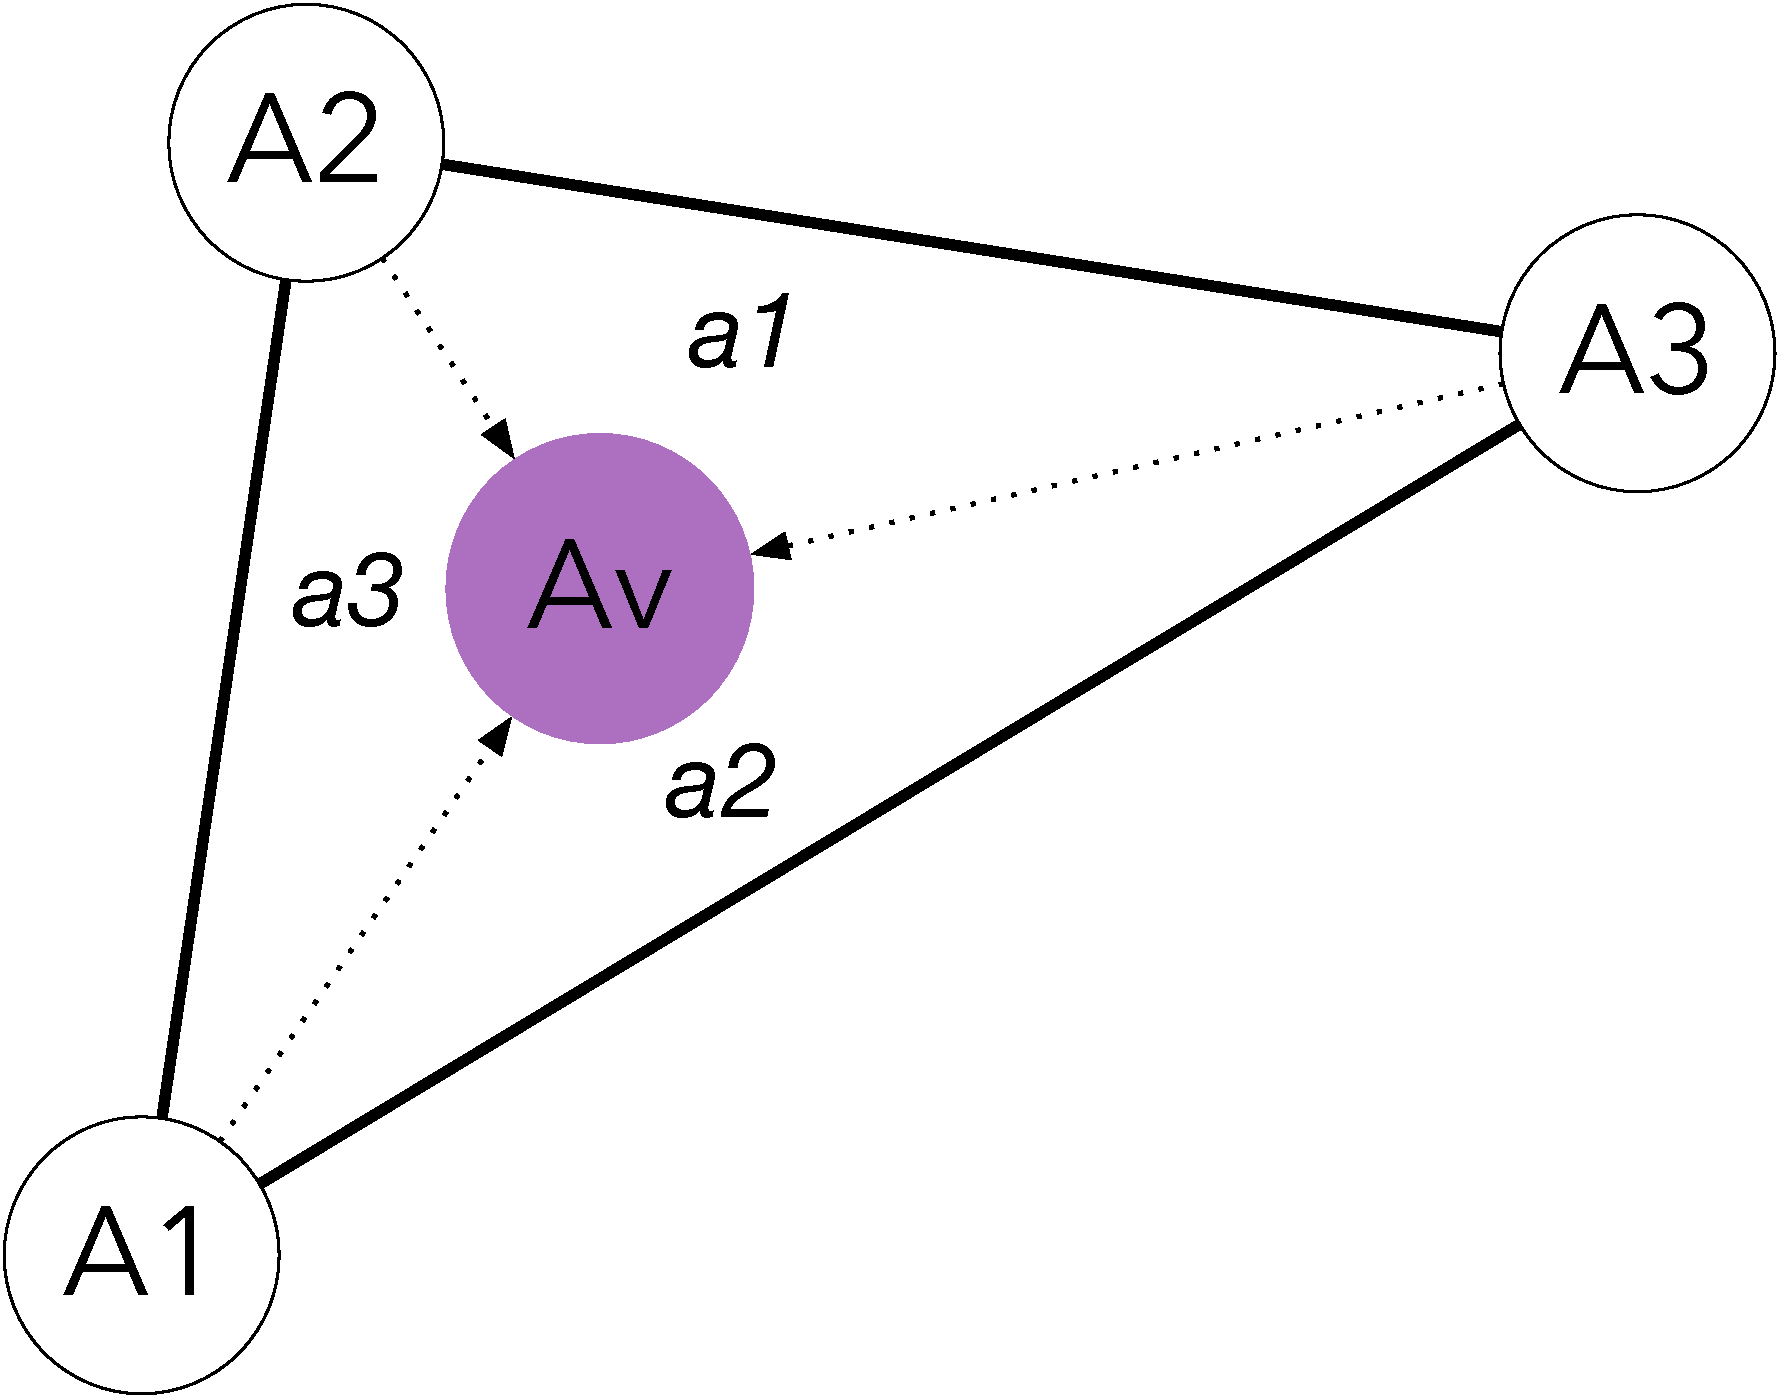
\includegraphics[width=0.8\textwidth, height=1.5in]{HA14-RenderingFigure-2015-01-17-2129} 
	   \caption{Barycentric coordinates.}
	   \label{fig:rendering:algorithm:barycentric}
    \end{subfigure}
    \qquad
     \begin{subfigure}[b]{0.4\textwidth}
       	\centering
	   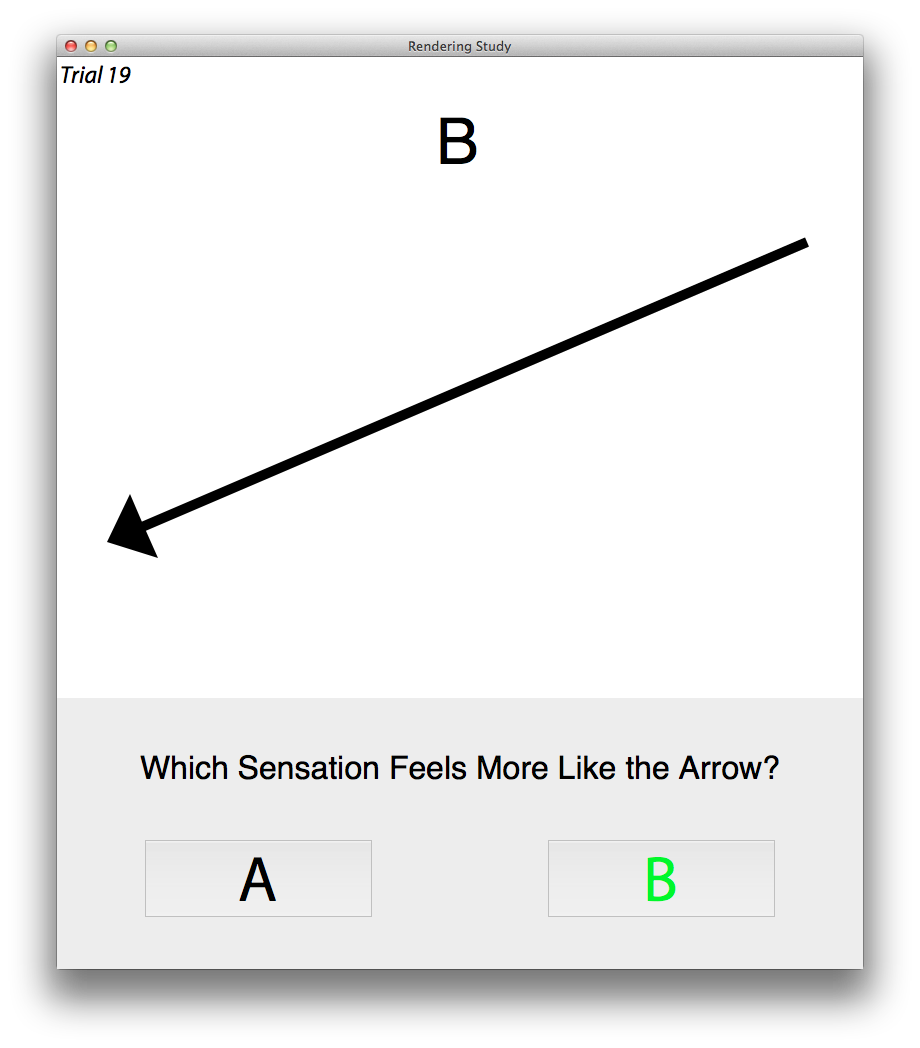
\includegraphics[width=0.6\textwidth, height=1.5in]{HA14-RenderingUI-2014-08-19-1417} 
	   \caption{Rendering study interface}
	   \label{fig:rendering:study}
    \end{subfigure}

    	   \caption{We ran a study to determine the preferred interpolation function to map barycentric coordinates (a1-3) to physical actuator output (A1-3) given a virtual intensity (Av).}
	   \label{fig:rendering:algorithm}
\end{figure}
%
%
%
%%%%%%%%%%%
%%
%%
%%
%%\subsection{Perceptual Study}
%
% Our first study is 
%We performed a pairwise comparison between the three candidate interpolation models prototyped for Mango's rendering pipeline.
%Our goal was to determine the user-preferred model for this VT hardware, to be used in Mango's ongoing implementation; and to identify relevant factors (e.g., frequency, amplitude, or individual differences).
%To determine the preferred model for this VT hardware in Mango's rendering pipeline, and to identify relevant factors (e.g., frequency, amplitude),%, or individual differences), 
We performed a pairwise comparison of our three candidate interpolation models.
Eighteen volunteers took part (6 female, between age 20-35). % aged 21 to 34) . 
%
%The VT hardware consisted of 10 high-quality VT actuators (C2 tactors, Engineering Acoustics, Inc., USA) arranged in a 3-4-3 layout and mounted on the back of a chair in a pad  21 cm high, 29 cm wide, and 2 cm thick;  actuators form equilateral triangles with edges of 6.35 cm  (\autoref{fig:rendering:device}). %The rendering engine updates at 100 Hz.
%\subsection{Results}
Analysis with stepwise regression revealed that logarithmic interpolation outperformed linear and was % found 
equivalent to Pacinian power model. We proceeded with the logarithmic model for Mango's implementation, as the power model did not outperform either of the others. % the linear model.
%Through piloting, we determined that the device's on-screen visual outline should mirror the sensations rendered on the physical device. That is, if participants see an animation object on the right side of the screen, they prefer to feel it on the right side of the back. 
% (as if they are looking from behind the VT hardware). 
\autoref{fig:rendering:study} shows the experiment interface, in which an arrow represents the sensation direction. 


\begin{figure}[t] %  figure placement: here, top, bottom, or page
   \centering
     \begin{subfigure}[b]{0.43\textwidth}
	   	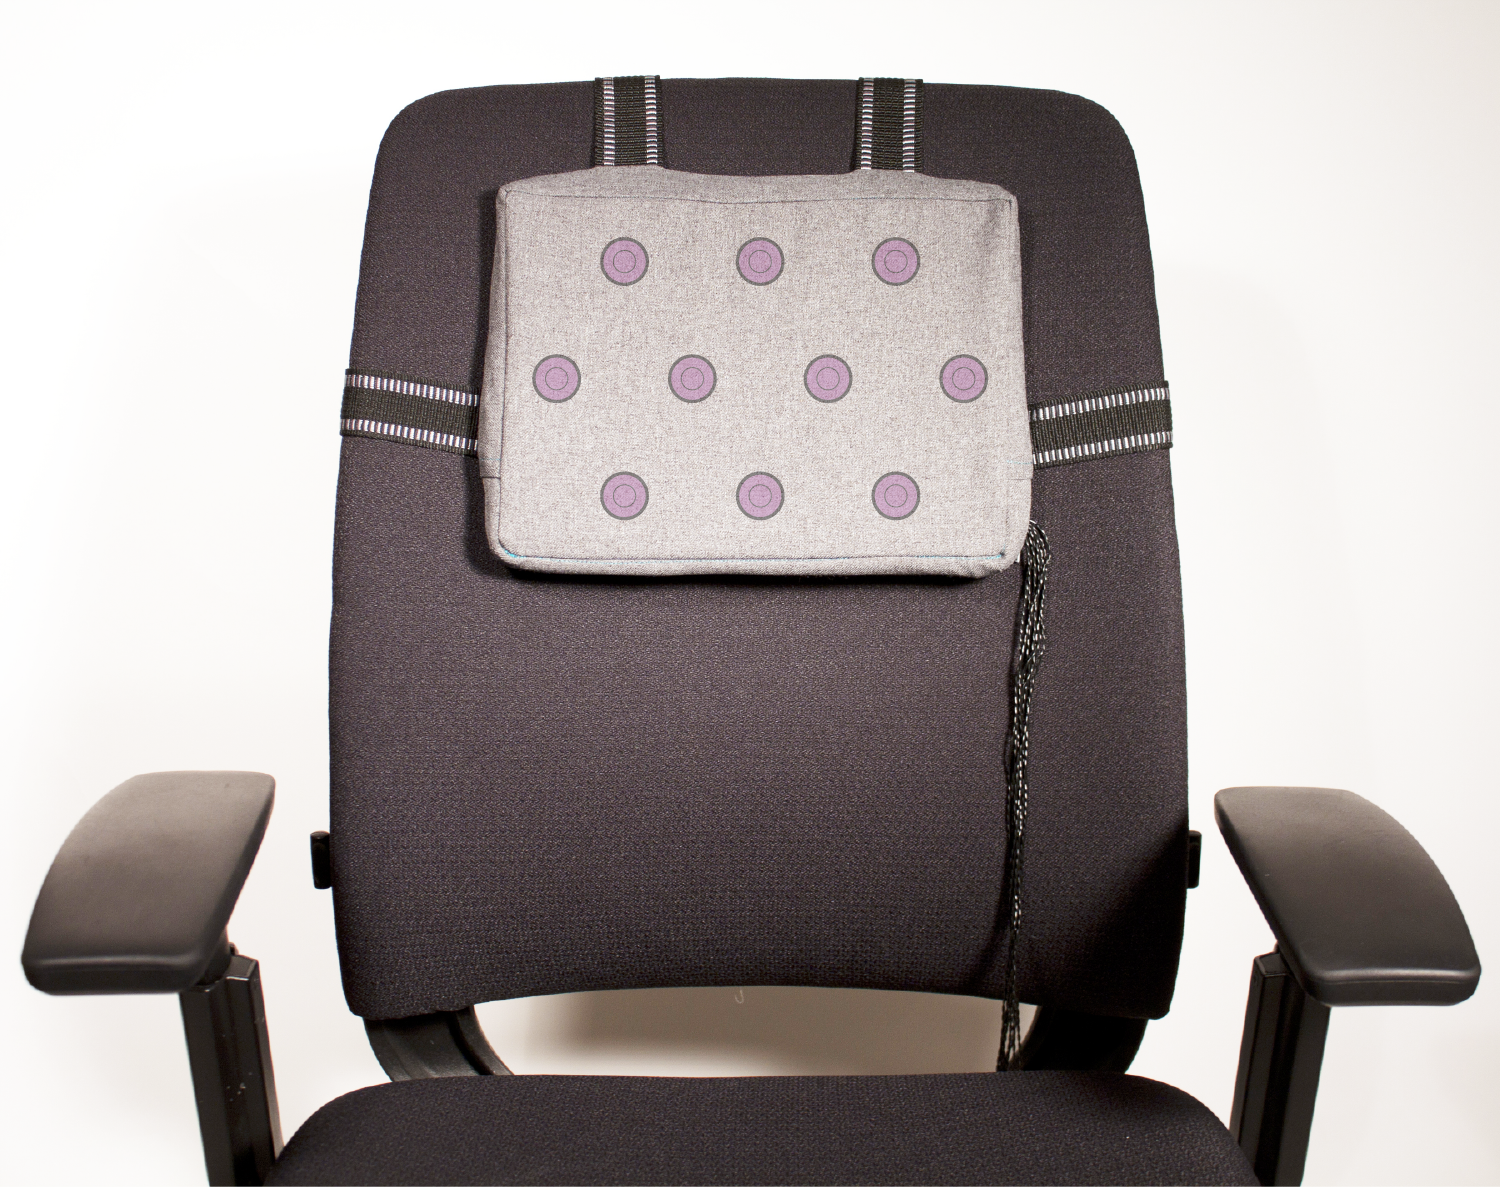
\includegraphics[width=\textwidth]{figure_chairpad} 
	   \caption{Output device with highlighted actuators}
	   \label{fig:rendering:device}
    \end{subfigure}
    \qquad
       \begin{subfigure}[b]{0.5\textwidth}
       		\centering
	   	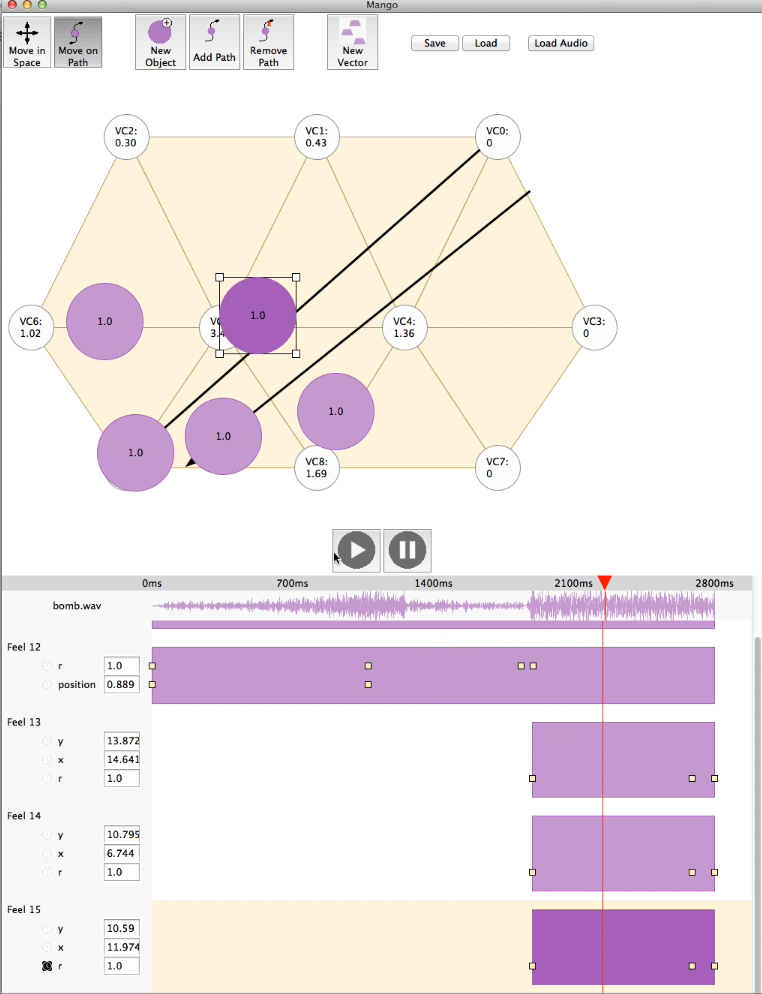
\includegraphics[clip=true, trim= 4 175 0 85, width=0.8\textwidth]{P2_sound_example-2014-09-22-1630} 
	\caption{Example of P2's animation for matching a sound.}
	\label{fig:animation:example:p2}
    \end{subfigure}
    	   \caption{Evaluation study setup and example design.}
	   \label{fig:rendering}
\end{figure}



%%%%%%%%%%
%
% Animation Tool Evaluation
%
\section{Design Evaluation}
% We implemented the critical functional features of Mango as described in the above sections.
To evaluate Mango's % the 
animation metaphor and expressive space with critical functional features implemented, we asked media professionals to
% we had media professionals 
create a variety of designs.
%, and qualitatively evaluated 
%its use for creating haptic content using both tactile animation objects (current design) and vector sensations (the state-of-the-art approach). 
%
%\subsection{Protocol}
Six participants (P1-6, 3 females) were introduced to Mango driving % linked to 
the  VT hardware described for the pairwise comparisons. 
%P1 had experience with haptics but not animation beyond video editing;
%P2-5 had animation experience but little or no experience with haptics;
%P6 had no experience with haptics or animation, but was familiar with media tools like Adobe Photoshop.
%P5 was also involved with the requirement gathering interviews presented earlier.
Each entire session took 40 to 60 minutes and consistened of a training task then three design tasks: design a heartbeat sensation, a ``turn left" sensation, and a sensation that matched a sound.
A semi-structured interview followed the design tasks informed by phenomenological protocols \cite{Moustakas1994}.
%The interviewer then followed up on interesting statements and/or concerns.
%During the interviews, participants were asked to compare animation objects with vector sensations, and to walk through the interface to elicit feedback.
%
% Study 2 results
%
%\subsection{Results}
Results were analyzed
% by considering each statement, memoing, coding, and relating codes
according to % Corbin and Strauss's 
grounded theory methods \cite{Corbin2008}, creating four themes.

%Each participant was introduced to Mango with a training task: % and the use of tactile animation objects and vector sensations.
%designing an alerting sensation using %  ``alert" sensation with 
%either animation objects or vector sensations (order counterbalanced).
%%half of them used the animation objects first and the other half used vector sensations first.
%Then, each participant was given three design tasks.
%1) Primarily \emph{temporal}: create a heartbeat sensation.
%2) Primarily \emph{spatial}: tell a driver to turn left.
%3) \emph{Context-based}: create a tactile animation to match a sound file.
%A 3-second sound effect of a bomb falling (with a whistle descending in pitch) then exploding with a boom was chosen, i.e., complex with with two semantic components.
%The wide array of resulting designs can be found in the accompanying video.
%

%
% Show one animation
%
%\begin{figure}[ht] %  figure placement: here, top, bottom, or page
%   \centering
%%   	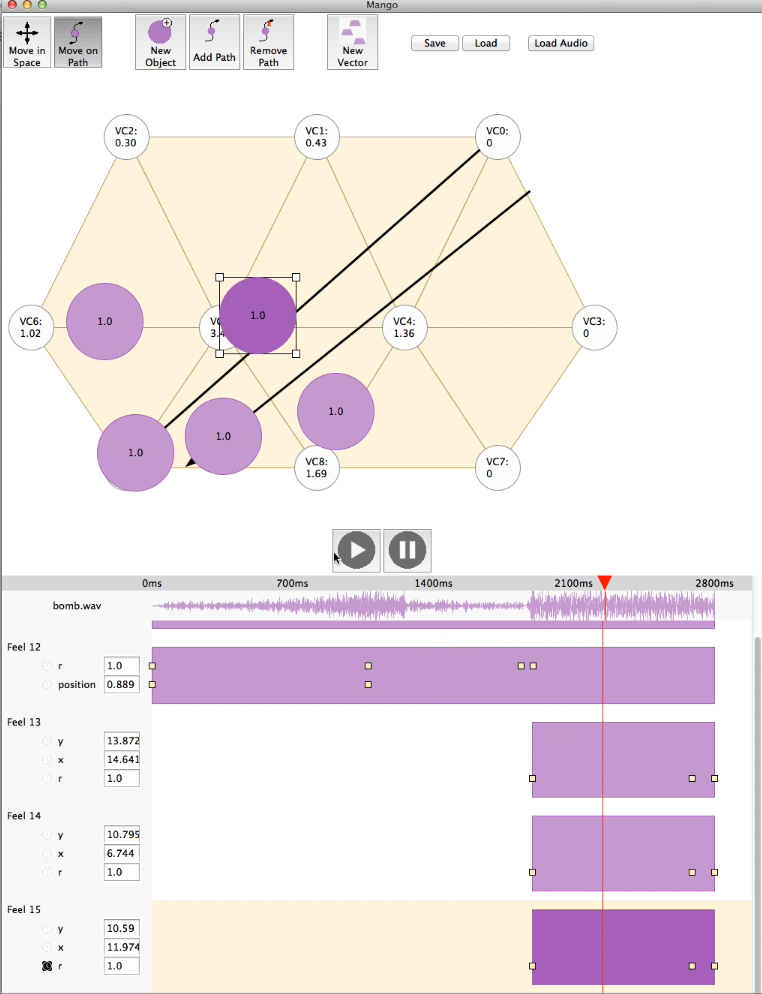
\includegraphics[clip=true, trim= 1 150 0 7, width=0.4\textwidth]{P2_sound_example-2014-09-22-1630} 
%	   	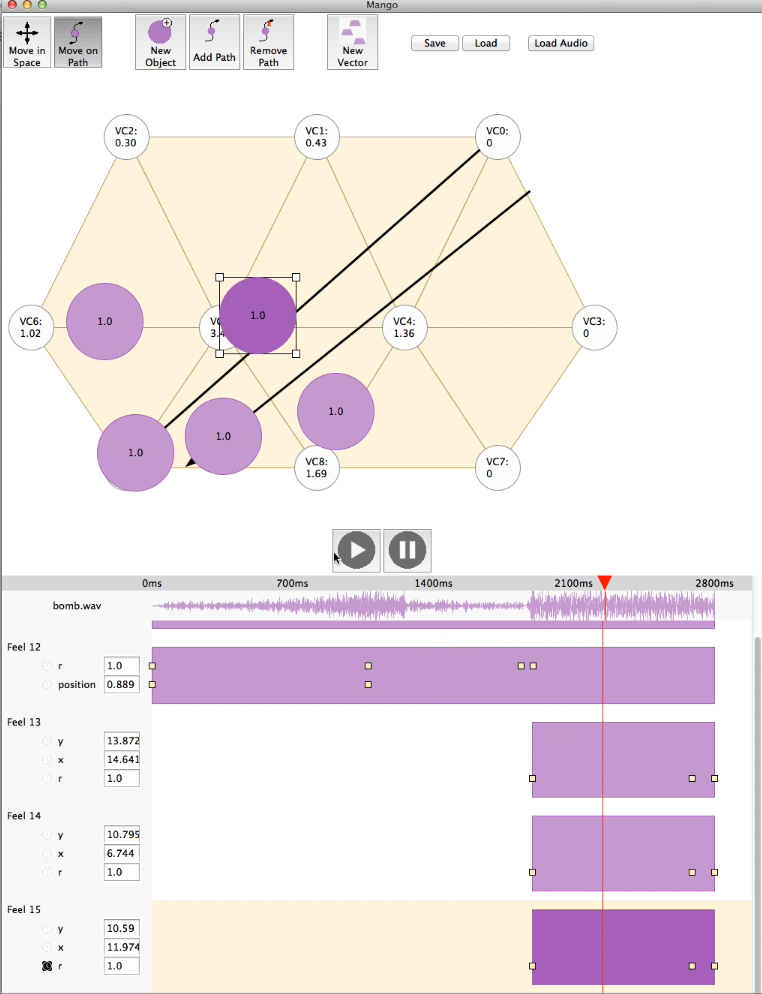
\includegraphics[clip=true, trim= 4 155 0 85, width=0.55\textwidth]{P2_sound_example-2014-09-22-1630} 
%
%	\caption{Example of P2's animation for matching a sound.}
%	\label{fig:animation:example:p2}
%\end{figure}




\textbf{Theme 1 - Animation Metaphor}
Participants found the tool easy to use.
All six participants were able to accomplish all five tasks (object alert, vector alert, heartbeat, turn left, sound) within their session.
%and described the interface as intuitive (P1-5), agreeing that it was an animation tool: \qq{It's up to the standards of other animation tools}{P1}, \qq{This is totally animation}{P2}, \qq{It felt very much like an animation tool}{P4}, \qq{I'm not an expert when it comes to haptics, but this software seems almost as if it can change the game of designing haptic vibrations}{P5}.
Negative feedback focused on polish and feature completeness.
%% not implementing enough features of their preferred tools and general feedback on polish and streamlining of the interface:
%\qq{gotta spline [the keyframe interpolation]}{P2}, \qq{a couple quirks but there was nothing difficult to overcome}{P4}, \qq{being able to design your own curve [path] would be really nice}{P5}, \qq{move in space and move on path can be one thing}{P6}.

\textbf{Theme 2 - Tactile Animation Object vs Vector Sensations}
Participants relied more on animation objects %  used animation objects more frequently
than vector sensations. %, which
%Vector sensations 
%were only used twice.%: P4's heartbeat task and P5's sound task (combined with an animation object).
%P1 switched from vectors to animation objects early in her heartbeat task;
%for her remaining tasks
%no other participants used vector sensations.
Animation objects were described as easier to use and more intuitive, especially to represent location or for non-animators.
%\qq{After using the new object I'd probably never use new vector again}{P2}, 
%%especially to describe motion or position:
%\qq{easier to find the location of the heart}{P1}, 
%%They were also described as more appropriate for people without animation experience:
%\qq{if I weren't an animator I think I would only use [animation objects]}{P4}.
%%, \qq{You have to be a little more careful when animating [vector sensations]}{P5}.
%%
%%Animation objects and vector sensations supported different workflows. Animation objects tended to be described as better for position, movement, and for % if you wanted to have 
%%multiple objects, while 
Vectors were preferred for more fine-tuned control when motion didn't matter as much, often using many keyframes.
%\qq{You can control multiple [actuators] at the same time, so you don't have to create new objects and then put them everywhere on the screen}{P1},
%\qq{[Animation objects] can be more comfortable to use when one doesn't work with keyframes}{P3}, 
%\qq{If you want precise control over [actuators], then vector is the way to go}{P4}.
%Participants rarely combined the two:
%\qq{I'm already into the object mode, I forget about the vector}{P6}.

%
% Shows three animations
%
%\begin{figure*}[htbp] %  figure placement: here, top, bottom, or page
%   \centering
%      	\begin{subfigure}[b]{0.30\textwidth}
%		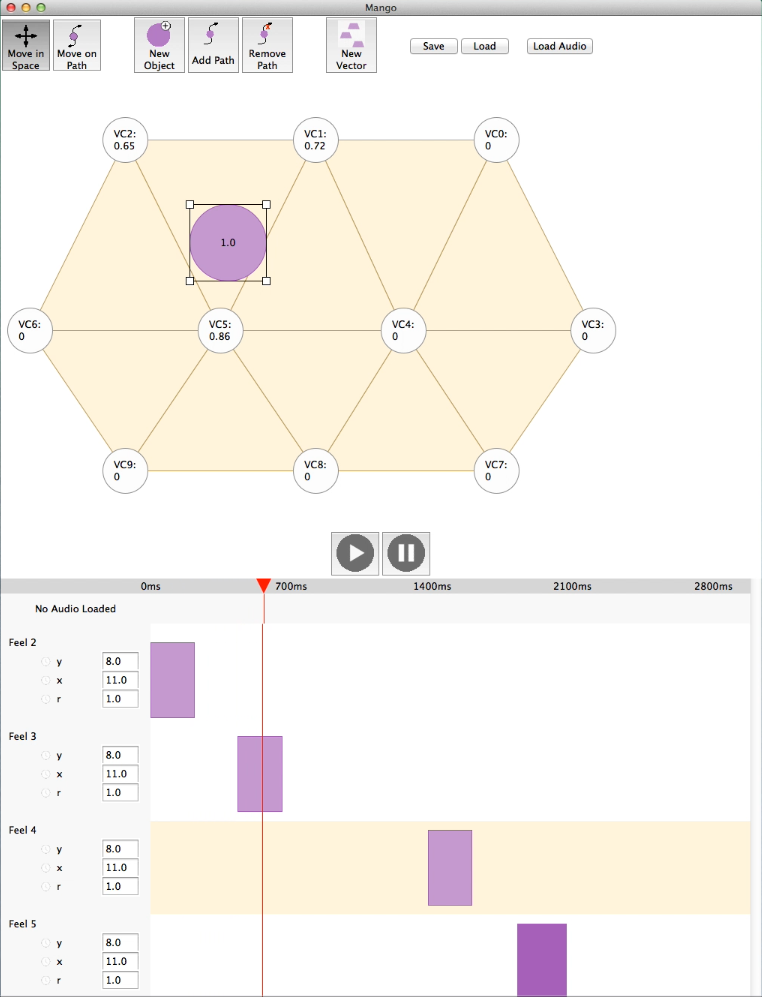
\includegraphics[width=\textwidth]{p1-heartbeat-example} 
%		\caption{Heartbeat task by P1}
%		\label{fig:animation:example:p1}
%	\end{subfigure}
%	\quad
%	\begin{subfigure}[b]{0.30\textwidth}
%		   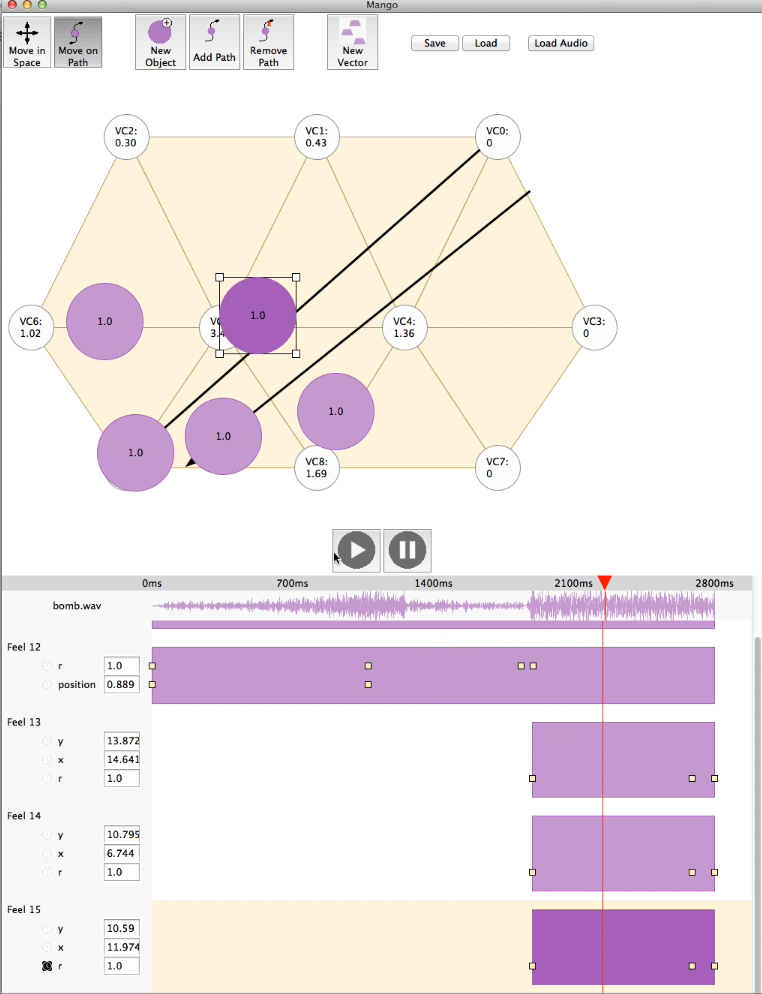
\includegraphics[width=\textwidth]{P2_sound_example-2014-09-22-1630} 
%		   \caption{Sound task by P2}
%		   \label{fig:animation:example:p2}
%	\end{subfigure}
%	\quad
%	\begin{subfigure}[b]{0.30\textwidth}
%		   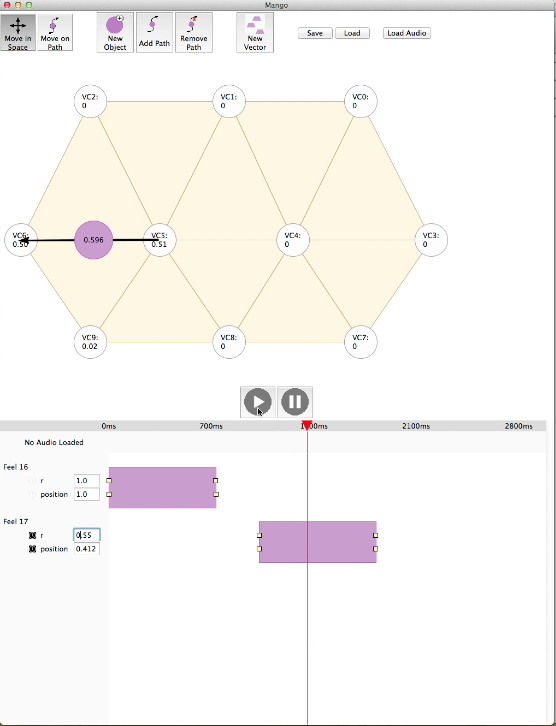
\includegraphics[width=\textwidth]{p4-turnleft-example-2015-01-19-1024} 
%		   \caption{Turn left task by P4}
%		   \label{fig:animation:example:p4}
%	\end{subfigure}
%
%
%
%
%      	\caption{Examples of Animations}
%	\label{fig:animation:example}
%\end{figure*}


%\theme{4}{Feedback, Context and Imitation}
%\theme{3}{Designing-in-action with direct manipulation}
\textbf{Theme 3 - Designing-in-action with direct manipulation}
Participants used direct manipulation to feel their designs in real time, %  was valuable to participants.
dragging animation objects %in the animation window
and scrubbing through
%at various speeds in
the timeline.
%: \qq{I would make the [animation] object and just play around with it before creating the animation, as a way to pre-visualize what I was going to do}{P5},
%\qq{I kind of play around with it, and randomly come up with the ideas}{P6}.
%P2 even noted that YouTube did not have
% real-time video scrubbing feedback like Mango's:
% %support for haptic and audio feedback:
% \qq{I wish I could scrub back and forth [with YouTube]}{P2}.
%However, continual % constant 
%vibrations were annoying, and participants requested a ``mute" feature:
%A VT feedback ``mute'' would be welcomed.
%P4 and P5 moved the timeline so that no output would play during design phase. 
% was playing while they were in design phase.
%\qq{It would be nice if when I [enter values into text fields] it doesn't go off constantly, it's getting annoying}{P3}.
%It was further suggested that each object should be independently mutable (as in hiding Photoshop layers), and VT output should be mutable entirely. 
More generally, participants used feedback from their experience or external examples.
P1 stopped to think about her heartbeat,  P2 used a YouTube video of a heartbeat as a reference, and P3 based her alert on her phone. %directly stated that she
%used imitation for the non-sound tasks
%;  her alert consisted of two vibrations similar to her phone: 
%\qq{It's typical to have two beeps for mobile phones}{P3}.
Similarly, participants were excited when prompted by an audio sensation.
%: \qq{I was really happy with the bomb one, because I could really hear it and imagine me watching a TV and then feel it at the same time}{P1},
%\qq{The sound part was good, that would be a fun thing to design for}{P4}.



%\theme{4}{Replication through Copy and Paste}
\textbf{Theme 4 - Replication through Copy and Paste}
Replication in both space and time was common while using Mango.
Many designs had symmetrical paths to reinforce sensations (\autoref{fig:animation:example:p2}).
All but P4 requested copy / paste as a feature.
%, suggesting it would be useful (P2, P3), faster (P1, P2) and easier (P5).
%P1, P2, and P5 wanted to duplicate their heartbeat sensation to be multiple beats, but did not do so without copy and paste.
%, instead saying they would repeat or loop it. [??????]
%\qq{I could just copy/paste the exact same thing on the left side and then move it to the right side}{P1}, \qq{I have the timing the way I like it, ideally it'd be cool if I was able to copy and paste these, so it would be able to repeat}{P5}.
%\qq{Is there any way to copy and paste keyframes?}{P2}.

%\section{Applications}



%\begin{figure}[htb] %  figure placement: here, top, bottom, or page
%   \centering
%   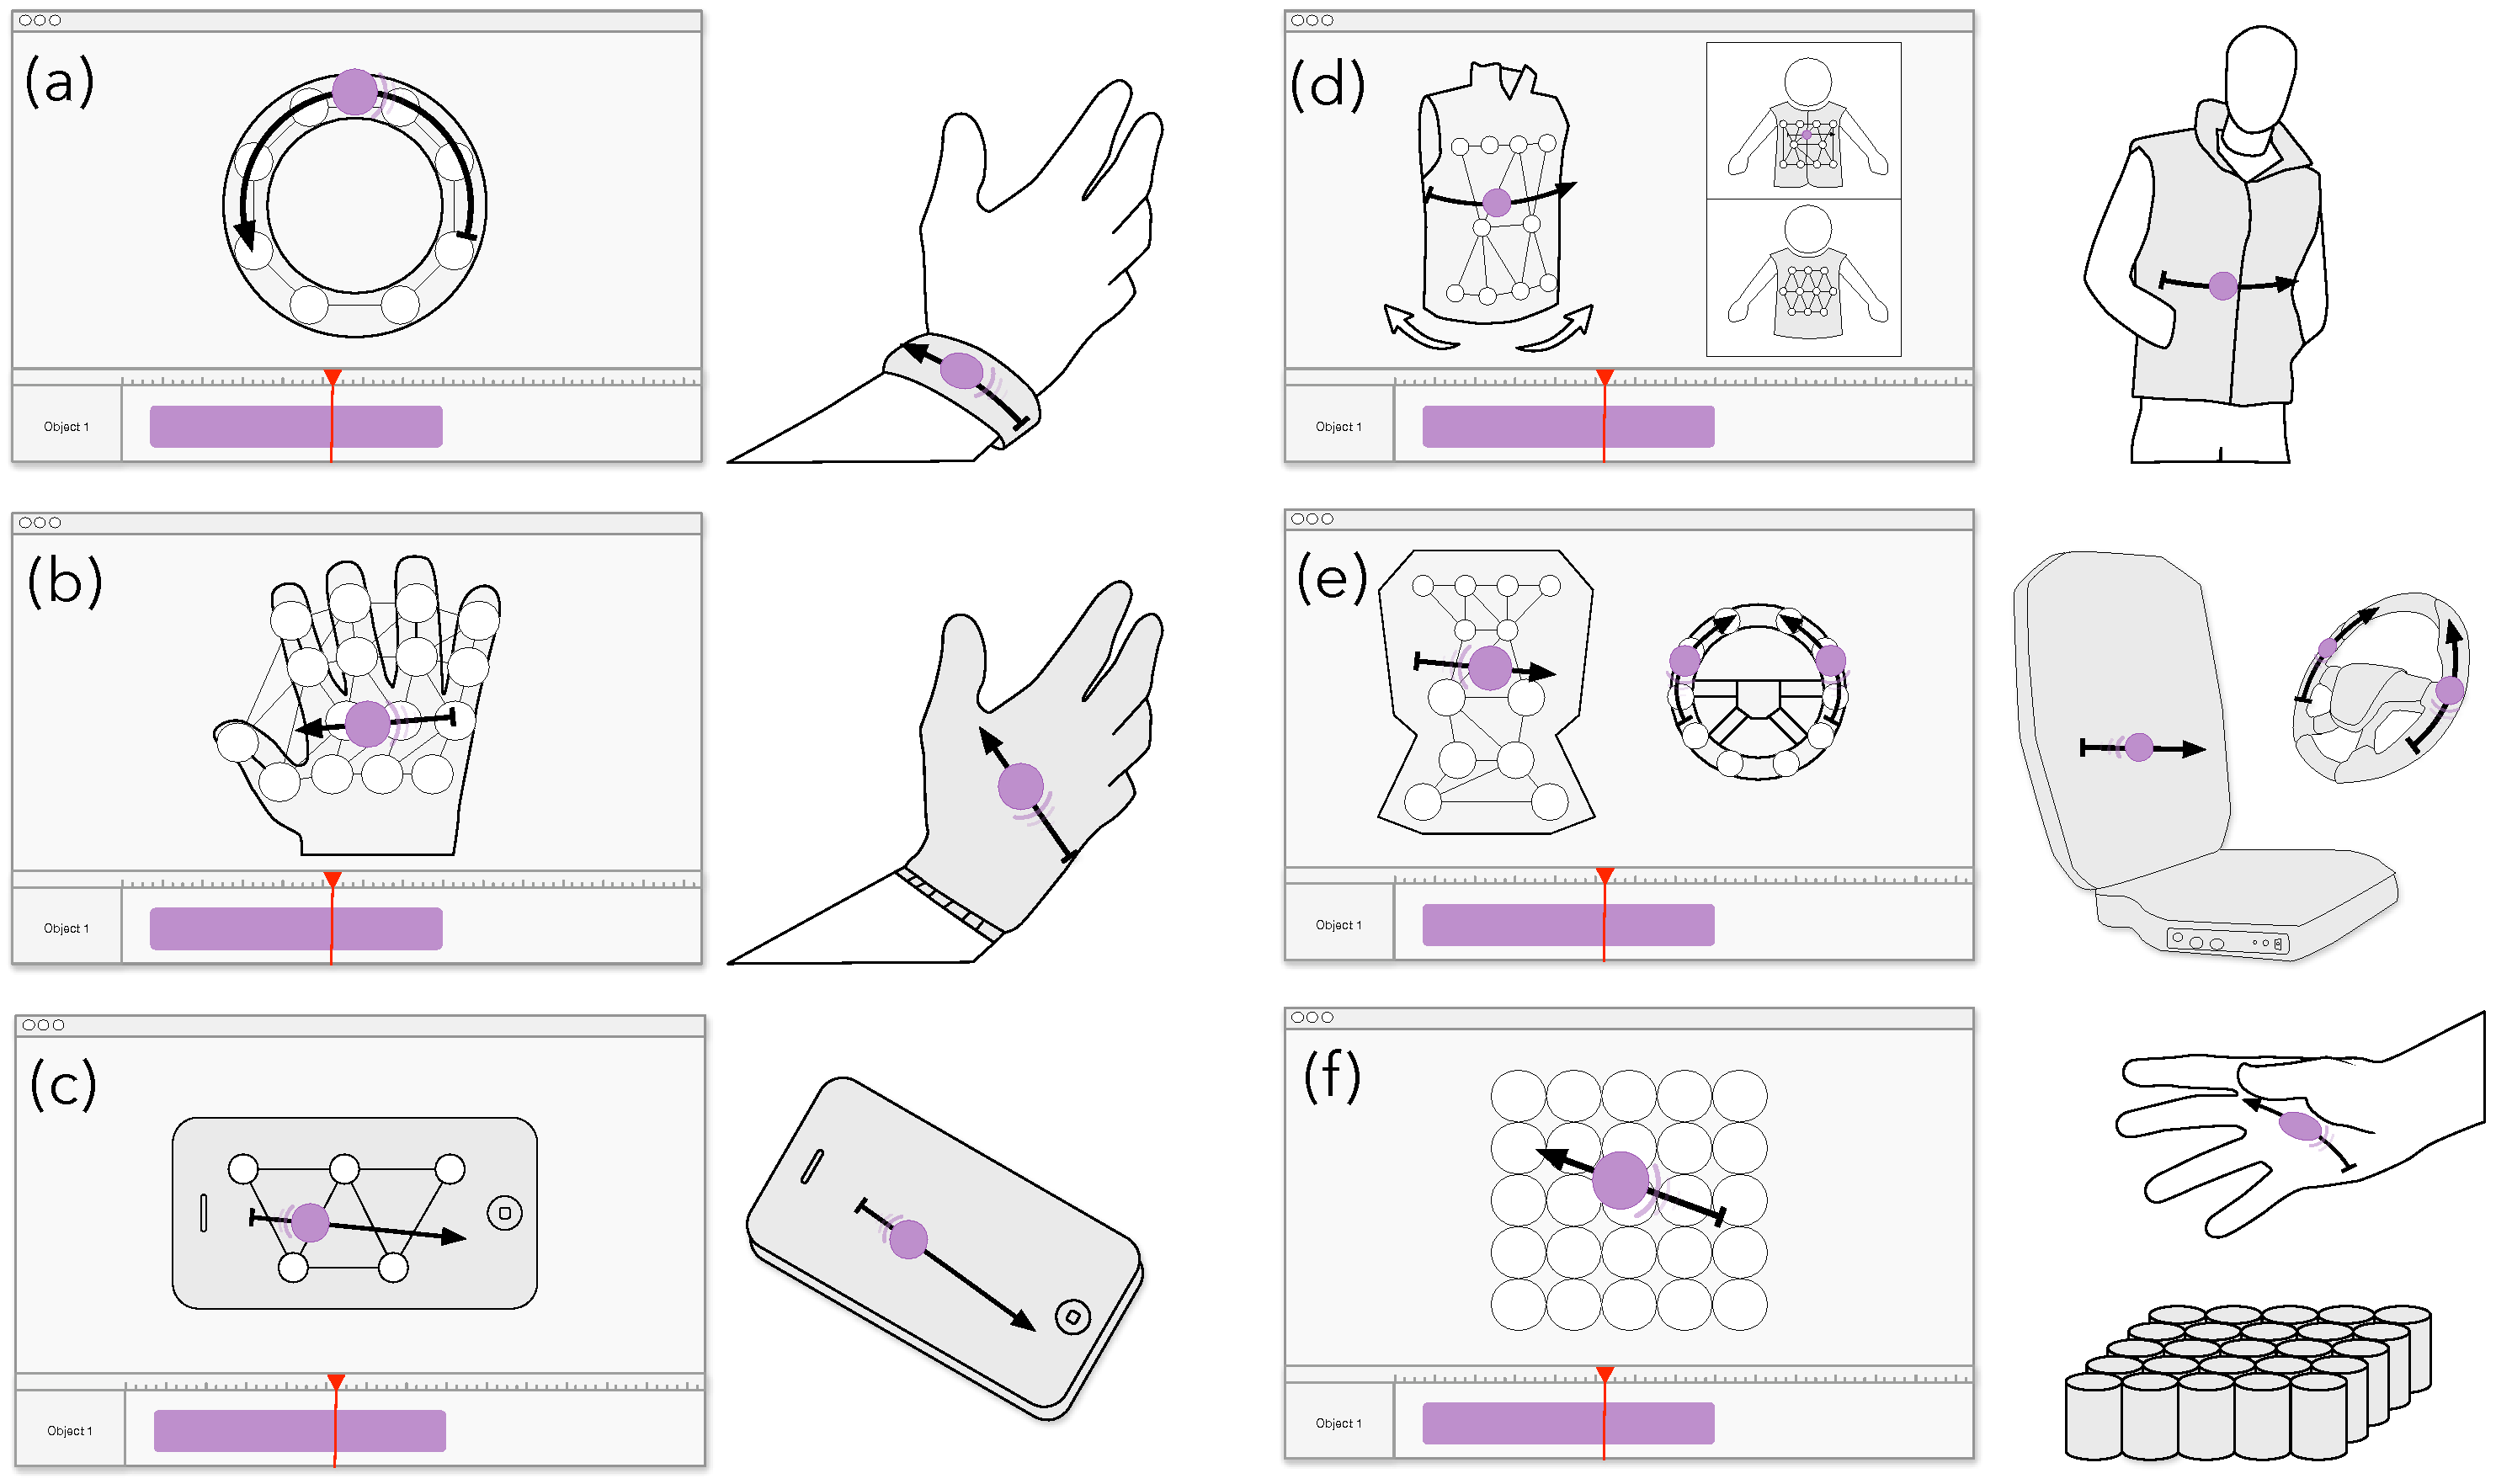
\includegraphics[width=0.8\textwidth]{HA14-Applications-SplitCombined-2015-04-14-1025} 
%   \caption{Tactile animation could define motion with (a) 1D actuator arrays, (b) dense and sparse VT grids, (c) handhelds, d)  3D surfaces, (e) multi-device contexts, and  (f) non-VT devices like mid-air ultrasound.}
%   \label{fig:application:space}
%\end{figure}

%\subsection{Design Evaluation Summary}
%From our design evaluation, we conclude that tactile animation is a promising approach for controlling haptic grid displays.
%Mango facilitated the design of a wide variety of animations (see accompanying video) and positive responses from participants.
%Direct manipulation of tactile animation objects supported embodied design and exploration by animators, who moved the objects to find the right location; this builds on results from the haptic instrument project.
%We also see several recommendations for our next iteration, adding more typical animation features, video as well as audio context, and muting.
%We build on this 

%The tactile animation metaphor also \kmC{orphan? Agree Discussion needs more oomph. Be sure to show balance - point out limitations, what its for vs what its not for, any criticisms raised by users. What stands between it and broader use?}

%%\subsection{Extension to Other Device Classes}
%The animation metaphor is a natural way to express spatial haptics.
%With additional rendering algorithms, some of which are known, we can generalize to other contexts.
%As long a single, spatio-temporal percept can be created, the animation metaphor can be used.
%See \autoref{fig:application:space} for sample applications.



%\vspace{20pt}

%\emph{1D VT Arrays (\autoref{fig:application:space1}a)}:
%1D VT arrays are common in arm sleeves, wrist bands, belts, and similar wearables.
%These devices provide sensations along the path of the array.
%By constraining objects to a linear or circular path, barycentric coordinates collapse into 1D interpolation.
%
%\emph{Dense and Sparse VT Grids  (\autoref{fig:application:space1}b)}:
%2D VT grids are also common, used in chairs, gloves, and the backs of vests.
%%Dense arrays previously had their own actuator-based authoring tools \cite{Kim2009}.
%While we evaluated Mango with a sparse back-mounted array, tactile animation naturally supports denser arrays, either with our rendering algorithm or by using a nearest-neighbour technique to activate a single actuator; in both cases, animation objects can be directly manipulated.
%%In the present work, we evaluated the usability of Mango to author variety of VT sensations on sparse arrays.
%%The actuator layout in both these devices are dif- ferent, and we accomodated them by selecting an appropriate
%%algorithm and layout to render high definition haptic feedback.
%
%
%\emph{Handhelds (\autoref{fig:application:space1}c)}:
%Actuators embedded in handheld objects such as mobile devices, game controllers, or steering wheels shake objects instead of directly stimulating the skin.
%Animators could define source locations for vibrations using handheld-based rendering algorithms (e.g., \cite{Seo2010}).
%%Similarly, a single embedded vibrator in handheld devices can be supported by constraining the tactile object to a single point.
%
%
%\emph{3D Surfaces  (\autoref{fig:application:space2}d)}:
%Mango currently only supports a 2D location for its animation objects.
%However, tactile animation can be extended to support surfaces of 3D surfaces, such as vests or jackets that wrap around the user's body. 
%More work will need to be done to perfect this interaction style, possibly using multiple views or a rotatable 3D model with animation objects constrained to the surface.
%%, drawing more from 3D animation tools like Maya.
%
%\emph{Multi-device contexts  (\autoref{fig:application:space2}e)}:
%Mango's rendering algorithm already supports connections to multiple devices simultaneously.
%The editing interface could combine layouts for different devices, enabling animators to animate the entire user experience (such as a car's seat and steering wheel).
%
%\emph{Non-vibrotactile devices (\autoref{fig:application:space2}f)}:
%While our rendering algorithm is particular to VT arrays, a tactile animation object can represent manipulable percepts with other actuation technologies.
%%Mango is not limited to only VT devices, similar to the one used in the present evaluations.
%Ultrasound-based mid-air displays generate a sensation as a focal point with a position and size \cite{Wilson2014}; this sensation could be manipulated through a tool like Mango.
%% produce a percept of object in mid-air and can be manipu- lated by changing the focal point as a animated object on the Mango interface. Algorithm to generate localize percept can be loaded along with the specifications written in the config- uration file.
%Similarly, passive force-feedback sensations (e.g., Hapseat \cite{Danieau2012a}) or height displays (a grid of pins) could be supported.
%


%\subsection{Interactive Applications}
%While our goal was enabling animators to create rich content, the tactile animation object can be linked to alternative input sources for other interactive experiences.
%
%\emph{User gestures.}
%User gestures and motion can be tracked and mapped to animation objects directly rendered on the haptic hardware.
%For example, a user creates pattens on a touch sensitive tablet that maps touch locations to a grid.
%Users could play games or create personalized haptic messages on the back of a vest.
%Similarly, a dancer's movements could be tracked through accelerometers, drawing animated haptic content on the body of her audience through actuated theater seats during a live performance.
%
%\emph{Camera feed extraction.}
%%Objects from Camera Feed
%Motion of objects from video feeds could be automatically extracted with computer vision and rendered on grid displays, providing dynamic patterns associated with actions during sports, movies, and games.
%Similarly, animation parameters from visual animation tools could be mapped to positions on a VT grid, creating haptic feedback for non-haptic media.
%
%\emph{Data streams.}
%One main application of haptic grid displays is to provide users directional, assistive, and navigational cues during driving cars, walking down the street, or with over-
%saturated sensory tasks.
%Users could associate digital data streams, such as GPS input, to predefined set of directional patterns on the back or palm of the hand.
%
%
%%\subsection{Limitations}
%%While the tactile animation metaphor can be naturally applied in many contexts, there are limitations.
%%Our perceptual study guided our development but does not constitute a full psychophysical investigation.
%%Further work needs to be done to identify the limits, thresholds, and peculiarities of this rendering technique.
%%Second, we only worked with triangular meshes, which might not be appropriate for all grids; quadrilateral interpolation or kernel methods could yield more convincing phantom sensations.
%%Finally, mixing actuator types (such as a chair with both voice coil and rumble motors, \autoref{fig:application:space2}e) could further generalize this approach.
%


\section{Discussion}
The Tactile Animation project expanded our understanding from the Haptic Instrument study in \autoref{ch:hapticinstrument}.
Specifically, it reaffirmed the value of real-time feedback and the need for examples, and showed that a persistent object model reduces cognitive load.
It also suggests again that examples and user experiences are extremely valuable to the design process, providing motivation for example-based haptic design discussed next in \autoref{ch:hapticexamples}.



%%%%%%%%%%
%
%Implications for Design
%
%%%%%%%%%%
%\section{Conclusion}
%
%%This paper presents Mango, a new tactile animation tool to create rich, dynamic and expressive haptic experiences. 
%%The tool utilizes animation metaphor in the design process and renders animated VT patterns on a variety of spatial VT displays.
%%Design requirements gathered in interviews and literature review are implemented on a prototype software that was evaluated with artists and a normal everyday computer user.
%%The post evaluation interviews and feedback suggested that the tool was useful and easily adaptable; and participants highly preferred animation metaphor to design haptic patterns.
%%Overall, tactile animation represents a promising new direction to support haptic media design.
%
%%A key feature of Mango is that it can be used with a wide range of haptic feedback hardware. The hardware specific definitions are provided in the configuration file which facilitates authoring of animations and its rendering on the hardware. Configuration files for new hardware can be constructed and loaded in Mango, to use its authoring capabilities with new hardware.  
%
%%\kmC{Adjust weight: tactile animation then Mango} % Km: up to here, I think it's consistent now. I ran out of steam.
%This paper introduces \emph{tactile animation}, a new approach for creating rich and expressive haptic media on grid displays.
%% The design of Mango is derived from an
%This animation metaphor allows designers and media artists to directly manipulate phantom vibrotactile sensations continuously in both space and time.
%Our rendering pipeline, which uses a perceptually-guided phantom sensation algorithm, enables critical real-time feedback for designing.
%%an approach that is more direct and potentially creative than coordinating individual actuators, and which scales better to large actuator maps, where perceived motion is nearly intractable using track-based approaches.
%%Unlike previous tools that either required rigorous programming background or was applicable to a specific hardware configuration, an animation approach also % our tool
%%provides a familiar interface to a large animation workforce, therefore eliminating training time and cost necessary for haptic content production in the mainstream media.  
%We incorporated these ideas into a prototype, Mango, with a design grounded in animator requirements and haptic design guidelines.
%Professional animators used our tool to create a variety of designs, giving positive feedback and excitement for future versions.
%This approach has the potential to % KM: concerned that this functionality can be added to any tool with properly designed configuration files, and isn't tied particularly to the other innovations reported here. If so, need to be much more careful about how it's phrased since this capability isn't even really demonstrated here - you only use one display apparatus.
%% Moreover, Mango 
%accommodate a large variety of haptic hardware, ranging from a single shaking element mounted on the seat to an array of actuators stimulating multiple points on the skin, and can export content into formats applicable in the production pipeline.
%Tactile animation empowers animators with a new set of artistic tools for rich, multimodal feedback. 
%
%\bibliographystyle{acmsiggraph}
%\bibliography{HA14-CHI2015,HA14-CHI2015-SIGGRAPH-add,verillo2}
\endinput
